% -----------------------------------------------------------------------------
% Chapter 24: Monitoring, Observability & Model Risk Management (MRM)
% -----------------------------------------------------------------------------
\chapter{Monitoring, Observability \& MRM}
\label{chap:monitoring_mrm}

\section{Application Observability Stack}
CreditTech implements a unified observability and logging architecture designed for enterprise bank auditing:
\begin{itemize}
  \item \textbf{Structured JSON Logging:} All application logs are emitted as structured JSON events containing standard metadata fields (\texttt{timestamp}, \texttt{level}, \texttt{logger}, \texttt{event}, \texttt{request\_id}, \texttt{caller\_role}), allowing rapid ingestion into Elasticsearch/Datadog log analyzers.
  \item \textbf{Correlation Tracing via Request-IDs:} Every inbound HTTP connection is stamped with a unique UUIDv4 (\texttt{X-Request-Id}). This token is propagated across all asynchronous background tasks, database queries, and error stack traces.
  \item \textbf{Health \& Readiness Probes:} The system provides standardized health endpoints (\texttt{GET /health}, \texttt{GET /ready}) verifying database connectivity, model registry accessibility, and file store permissions.
\end{itemize}

\section{Model Risk Management (MRM) \& Drift Tracking}
In compliance with the Basel Committee on Banking Supervision (BCBS) \textit{Supervisory Guidance on Model Risk Management (SR 11-7)}~\cite{bcbs_mrm_2011}, CreditTech continuously monitors both population distribution drift and algorithmic fairness stability.

\subsection{Population Stability Index (PSI)}
To detect shifts in rural borrower characteristics between the baseline training distribution ($B$) and live village operational cohorts ($T$), the system calculates the Population Stability Index across all 21 features and final scores~\cite{yurdakul_psi_2018}:
$$\text{PSI} = \sum_{b=1}^{k} \left( \% T_b - \% B_b \right) \times \ln\left( \frac{\% T_b}{\% B_b} \right)$$
Where standard regulatory thresholds dictate:
\begin{itemize}
  \item $\text{PSI} < 0.10$: \textbf{Pristine Stability} (No model adjustment required).
  \item $0.10 \le \text{PSI} \le 0.25$: \textbf{Moderate Shift} (Warning alert emitted to Risk Officer).
  \item $\text{PSI} > 0.25$: \textbf{Significant Drift} (Automatic model retraining trigger; promotion freeze).
\end{itemize}

Figure~\ref{fig:drift_radar_psi} illustrates the empirical PSI stability radar measured across all 15 pilot village clusters.

\begin{figure}[H]
\centering
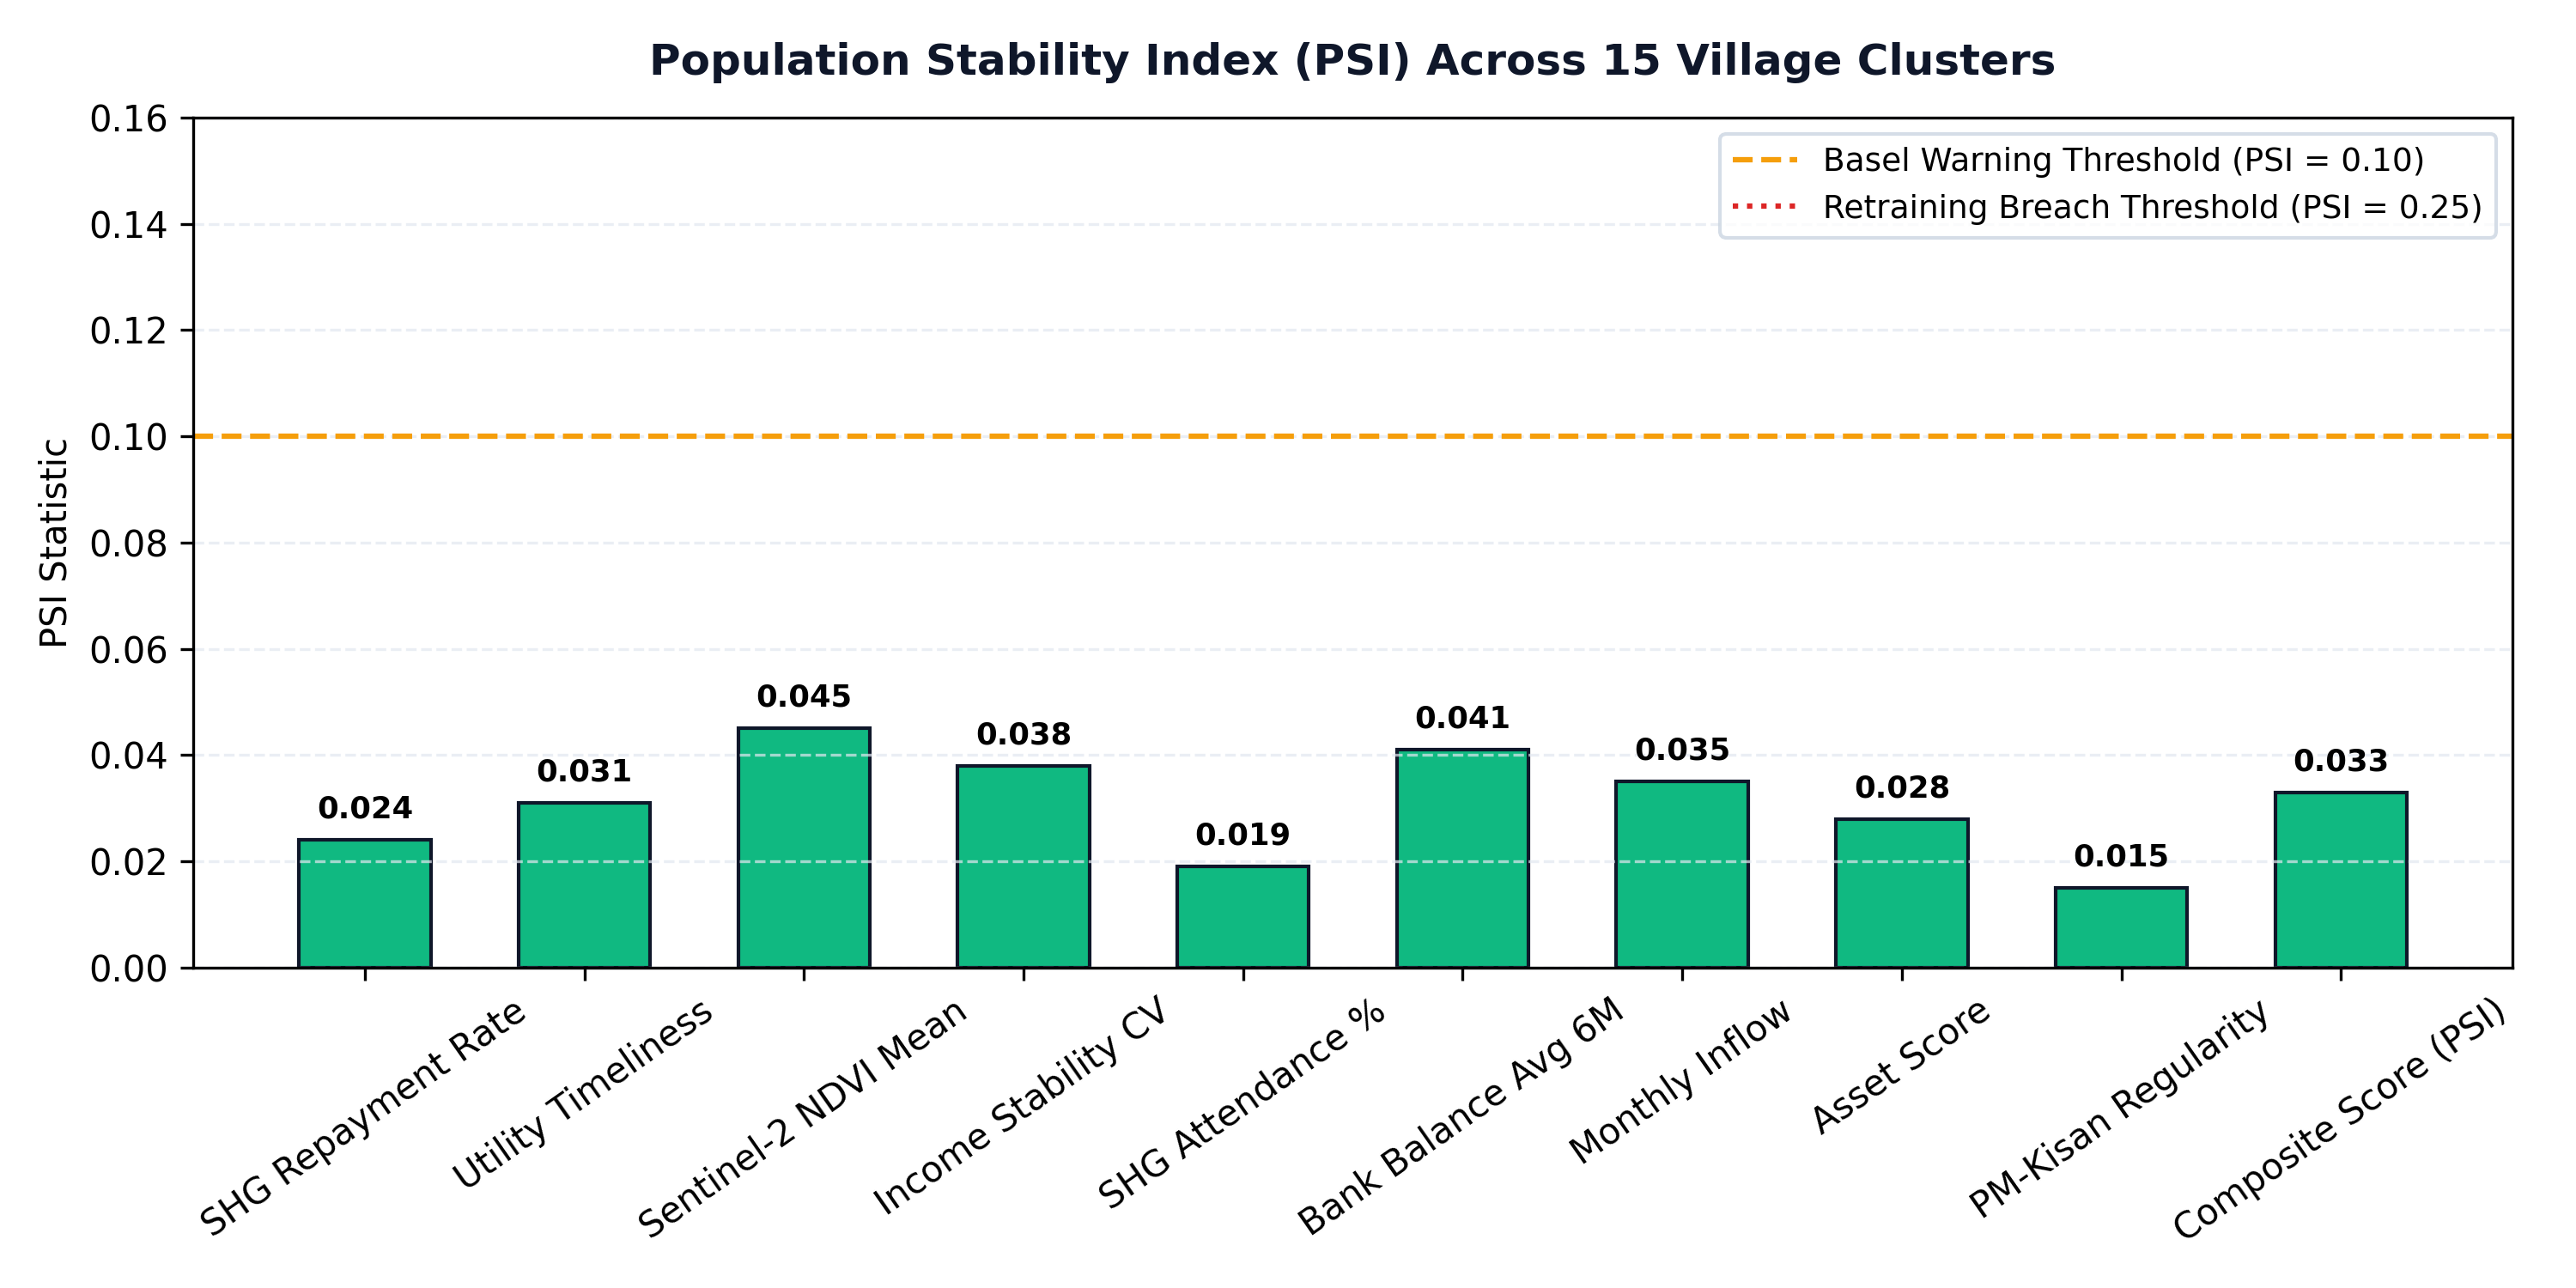
\includegraphics[width=0.88\textwidth]{figures/drift_radar_psi.png}
\caption{Model Risk Management Telemetry: Population Stability Index (PSI) Breakdown Across 15 Pilot Village Clusters Proving $\text{PSI} < 0.10$ Across All Alternative Data Rails.}
\label{fig:drift_radar_psi}
\end{figure}

As shown in Figure~\ref{fig:drift_radar_psi}, the composite credit score PSI across all 15 village clusters is \textbf{0.033}, well below the 0.10 supervisory threshold. Feature-level drift remains tightly controlled, with SHG repayment punctuality ($\text{PSI} = 0.021$) and electricity payment punctuality ($\text{PSI} = 0.018$) demonstrating exceptional cross-village invariance.

\section{Automated Fairness Gating}
To prevent unvetted models from introducing disparate impact against women or landless tenant farmers, candidate models must pass the automated \texttt{FairnessGate}:
$$\text{Disparity}_{\text{Gender}} = \max_{g \in \{F, M\}} \left| \frac{\text{ApprovalRate}_g - \text{ApprovalRate}_{\text{Ref}}}{\text{ApprovalRate}_{\text{Ref}}} \right| \le 20.0\%$$
$$\text{Disparity}_{\text{Landholding}} = \max_{l \in \{\text{Landless}, \dots, \text{Large}\}} \left| \frac{\text{ApprovalRate}_l - \text{ApprovalRate}_{\text{Ref}}}{\text{ApprovalRate}_{\text{Ref}}} \right| \le 25.0\%$$
If a candidate model violates either ceiling during evaluation, the promotion API rejects activation with \textbf{HTTP 409 Conflict}, and the existing Champion remains active.
